%! Author = nadutkinfedor
%! Date = 14.01.2024

% Preamble
\documentclass[11pt]{article}
\usepackage[left=2cm, right=1cm, top=2cm, bottom=2cm, bindingoffset=0cm]{geometry}

% Packages
\usepackage[utf8]{inputenc}
\usepackage[russian]{babel}
\usepackage{amsmath}
\usepackage{hyperref}
\usepackage{graphicx}
\usepackage{misccorr}
\usepackage{listings}
\usepackage{xcolor}
\usepackage{titlesec}
\usepackage{minted}
\usepackage{color}
\usepackage{enumitem}
\usepackage{indentfirst}

%listing settings
\definecolor{dkgreen}{rgb}{0,0.6,0}
\definecolor{gray}{rgb}{0.5,0.5,0.5}
\definecolor{mauve}{rgb}{0.58,0,0.82}

\lstset{ %
    backgroundcolor=\color{white},   % choose the background color
    basicstyle=\footnotesize,        % size of fonts used for the code
    breaklines=true,                 % automatic line breaking only at whitespace
    captionpos=b,                    % sets the caption-position to bottom
    commentstyle=\color{dkgreen},    % comment style
    escapeinside={\%*}{*},          % if you want to add LaTeX within your code
    keywordstyle=\color{blue},       % keyword style
    stringstyle=\color{mauve},     % string literal style
}

% Title
\title{Параллельные алгоритмы}
\author{Надуткин Федор }
\date{January 2023}

\titleformat{\section}[block]{\Huge\bfseries\filcenter}{}{1em}{}
\titleformat{\subsection}[block]{\huge\bfseries\filcenter}{}{1em}{}
\titleformat{\subsubsection}[block]{\Large\bfseries\filcenter}{}{1em}{}

% Document
\begin{document}

    \maketitle
    \newpage

    \section*{Параллельные алгоритмы}

    \begin{figure}[h!]
        \includegraphics*[width=0.9\textwidth]{Pictures/Parallel and Concurrent Algorithms}
        \caption{Параллельные и конкурентные алгоритмы}
        \label{fig:parallel_and_concurrent}
    \end{figure}

    Разница между параллельными и конкурентными алгоритмами в том,
    что у параллельных алгоритмов вход и последующая работа синхронизирована, и им не нужно конкурировать за ресурсы,
    а надо лишь распараллеливать уже имеющуюся работу,
    тогда как у конкурентных такой синхронизации нет, и им нужно дополнительно о ней заботиться.

    \section*{PRAM}

    \begin{figure}[h!]
        \centering
        \includegraphics*[width=0.5\textwidth]{Pictures/PRAM/PRAM}
        \caption{Parallel Random Access Machine}
        \label{fig:pram}
    \end{figure}

    Изначально была придумана модель PRAM, в которой все операции были разбиты на шаги,
    и каждый такт $n$ процессов выполняли один из шагов $1, 2, \dots, k$.
    Однако в скоре стало ясно, что такая модель достаточно дорогая и требует синхронизации для $n$ потоков каждого шага.

    Среди возможных операций были \textbf{read(x)} - чтение, \textbf{write(x, y)} - запись и \textbf{arithmetic} - арифметические операции.
    Как следствие возникают различные уровни доступа.
    \begin{itemize}
        \item \textbf{EREW} - Exclusive reads, Exclusive writes.
        В каждый момент времени переменную могут либо читать, либо писать, и только лишь один поток.
        \item \textbf{CREW} - Concurrent read, Exclusive write.
        В каждый момент времени несколько процессов могут читать переменную, но лишь один может писать.
        \item \textbf{CRCW} - Concurrent reads, Concurrent writes.
        Во время записи будет один победитель, значение которого запишется.
        \begin{itemize}
            \item \textit{common} - Все процессы пишут одинаковое значение.
            \item \textit{priority} - Запишется значение приоритетного потока.
            \item \textit{random} - Запишется значение рандомного потока.
        \end{itemize}
    \end{itemize}

    \textbf{Work} - сколько работы было сделано.
    В PRAM это $n \cdot k$

    \textbf{Time} - сколько времени работал алгоритм.
    В PRAM это $k$

    CRCW можно проэмулировать на EREW, однако Time станет равным $k \cdot \log{n}$.
    На каждом шаге у нас есть $n$ процессов, мы делаем операции write во временные ячейки,
    после чего мы начинаем их агрегировать, что можно сделать за $\log{n}$ времени.

    Пример приведён на рисунке.

    \begin{figure}[h!]
        \centering
        \includegraphics*[width=0.7\textwidth]{Pictures/PRAM/CRCW from EREW}
        \caption{Перевод из EREW в CRCW}
        \label{fig:erew_to_crcw}
    \end{figure}

    Алгоритм работы PRAM можно видеть ниже.
    Здесь мы считаем сумму элементов в массиве.
    Количество элементов равно количеству потоков, равно $n$.
    \texttt{Time} $= \log{n}$, \texttt{Work} $= n \cdot \log{n}$.

    \begin{lstlisting}[label={lst:array_sum},caption={Пример подсчёта суммы элементов в массиве}]
        id
        read(a, A[id])
        write(B[id], a)
        for h = 1...log(n):
            if id <= n / (2^h):
                read(B[2 * id - 1], x)
                read(B[2 * id], y)
                z = x + y
                write(B[id], z)
            else:
                skip(4)
    \end{lstlisting}

    Однако стоит заменить, что у нас на каждом шаге работают лишь $\frac{n}{2^h}$ процессов, как следствие есть идея заменить такую структуру на \texttt{pfor}.

    \begin{lstlisting}[label={lst:pfor}, caption={Работа pfor}]
        for h = 1...log(n):
            pfor i = 1...n/(2^h):
                read(B[2 * id - 1], x)
                read(B[2 * id], y)
                z = x + y
                write(B[id], z)
    \end{lstlisting}

    Однако в реальных моделях создать \texttt{pfor} за один такт достаточно проблематично и дорого,
    поэтому появилась модель \texttt{fork-join}, которая порождает лишь 2 потока за раз.

    В реальной жизни модель \texttt{Time} уже не подходит,
    время будет сильно зависеть от машин, от того что делается в каждом \texttt{fork-join} \ldots,
    поэтому \texttt{Time} заменяется на \textbf{Span} - глубину графа.

    \begin{figure}[h!]
        \centering
        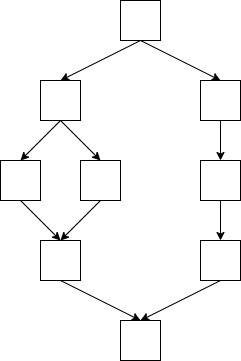
\includegraphics[width=0.3\textwidth]{Pictures/SPAN}
        \caption{Пример работы fork-join}
        \label{fig:fork_join}
    \end{figure}

    На изображении выше \texttt{Work} $= 9$, а \texttt{Span} $= 5$.
    Для составления такого графа нужны планировщики.

    \subsection*{Теорема Брента}

    Время работы \texttt{level-by-level} планировщика $T \leq \frac{W}{p} + S$,
    где $W$ --- \texttt{Work}, $S$ --- \texttt{Span}, $p$ --- количество потоков.

    \textbf{Доказательство}

    На каждом уровне время работы $= \lceil \frac{W_i}{p} \rceil$,
    всего уровней у нас \texttt{Span}.
    Суммарное время работы $T = \lceil \frac{W_1}{p} \rceil + \lceil \frac{W_2}{p} \rceil + \dots \lceil \frac{W_s}{p} \rceil \leq \frac{W_1}{p} + 1 + \frac{W_2}{p} + 1 + \dots + \frac{W_s}{p} + 1 = \frac{W_1 + W_2 + \dots + W_s}{p} + S$

    \subsection*{Теорема}

    $\forall$ \texttt{greedy-scheduler} $T \leq \frac{W}{p} + \frac{p-1}{p} \cdot S$

    \textbf{Доказательство:}

    \begin{figure}[h!]
        \centering
        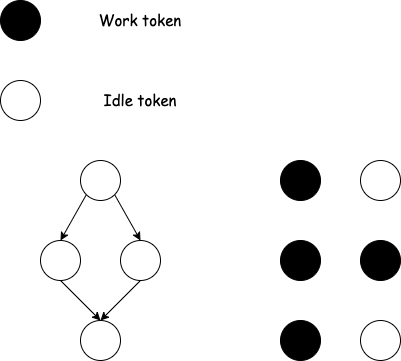
\includegraphics[width=0.5\textwidth]{Pictures/Greedy Scheduler}
        \label{fig:greedy_scheduler}
    \end{figure}

    Введём определения
    \begin{itemize}
        \item \texttt{Work Token} - платим, когда мы работаем.
        \item \texttt{Idle Token} - платим, когда мы отдыхаем.
    \end{itemize}

    Когда мы платим хотя бы один \texttt{Idle Token} наш \texttt{Span} уменьшается на 1.
    За каждый уровень мы платим $\leq S \cdot (p - 1)$ (хотя бы один процесс должен работать).
    Так как каждую итерацию нам приходит $p$ токенов (у нас $p$ процессов), то $T \leq \frac{W}{p} + \frac{p-1}{p} \cdot S$

    Как следствие $T \leq \frac{W}{p} + S$, а значит брать $p \geq \frac{W}{S}$ имеет мало смысла.
\end{document}